\documentclass[usenames,dvipsnames]{beamer}
\mode<presentation>{}
\usetheme{ULB}


\newcounter{FootlineChoice}
\newcounter{DepartmentLogo}
\newcounter{FacultyLogo}

\def\DepartmentLogo{theme/logos/urlab.pdf}
% In the folder "theme/logos/" please import the Department logo image. This will appear at north east corner of every frame

\setcounter{DepartmentLogo}{2}
% Please select 0 if you want a blank NE corner for each frame
% Please select 1 if you want the Department Logo only on the Title Page (NE corner)
% Please select 2 if you want the Department Logo on each frame (still NE corner)


\def\FacultyLogo{theme/logos/ulb_sciences.png}
% In the folder "theme/logos/" please import the Faculty logo image. This will appear at south east corner of title frame

\setcounter{FacultyLogo}{1}
% Please select 1 if you want the Faculty Logo to be displayed in the sE corner of the title frame
% Please select 0 if you want a blank SE corner for the title frame


%%%%%%%%%%%%%%%%%%%%%%%%%%%%%%%%%%%%%%%%%%%%%%%%% FOOTLINE MANAGEMENT %%%%%%%%%%%%%%%%%%%%%%%%%%%%%%%%%%%%%%%%%%%%%%%%%

\setcounter{FootlineChoice}{3}
% Please select value 0,1, or 2 for the footline alignment.
% All footlines display the [author] in SW corner and [institute] in SE corner,
% but you can choose between the following options for the center of the footline :

% Footline Aligment 0 : 
%       Only the current section is displayed. All is aligned with the very bottom of the frame.

% Footline Aligment 1 :
%       Only the current section is displayed. All is aligned a bit higher to escape potential crops when projecting.

% Footline Aligment 2 : 
%       Current section and subsection are displayed.  All is aligned a bit higher to escape potential crops when projecting.

% Footline Alignment 3 :
%       Nothing displayed at center. [author] and [institute] aligned with very bottom of frame.

\usepackage{xcolor}
\usepackage{caption}
\usepackage{subcaption}
\usepackage{multimedia}
\usepackage{soul}
\usepackage{svg}
\usepackage{listings}
\usepackage{inconsolata}

%add support for unicode \ding{55} and \ding{51}
\usepackage{pifont}
\newcommand{\greenv}{\textcolor{ForestGreen}{\ding{51}}}
\newcommand{\redx}{\textcolor{red}{\ding{55}}}
\newcommand{\backupbegin}{
	\newcounter{finalframe}
	\setcounter{finalframe}{\value{framenumber}}
}
\newcommand{\backupend}{
	\setcounter{framenumber}{\value{finalframe}}
}


\title{Git 101:\\ Tout ce qu'il faut connaitre pour etre un bon dev.}
\subtitle{Atelier Git(hub)}
\date{\today}
\author{Kevin \textsc{Vandervaeren}}
\institute{ULB -- URLAB}


\begin{document}

\begin{frame}[plain,noframenumbering]
	\titlepage
\end{frame}

\begin{frame}{Agenda}
	\begin{columns}
		\begin{column}{0.65\linewidth}
			\begin{itemize}
				\item<1-> donné et partage de fichiers 
				\item<2-> Introduction à Git
				\begin{itemize}
					\item comment ça marche ?
					\item quel sont les avantages ?
					\item comment l'installer ?
					\item comment l'utiliser ?
					\item exercices pratiques
				\end{itemize}
				\item<3-> Introduction à GitHub (ou autre plateforme)
				\begin{itemize}
					\item En quoi est-ce différent de Git ?
					\item Comment l'utiliser ?
					\item avantages et inconvénients
					\item exercices pratiques
				\end{itemize}
				\item<4-> Conclusion et synthèse
				\item<5-> Et pour aller plus loin
			\end{itemize}
		\end{column} %%
		\begin{column}{0.3\linewidth}
			
\includegraphics[width=\linewidth]{Im/Git-logo.png}
		\end{column}
	\end{columns}
\end{frame}

\begin{frame}[fragile]{donné et partage de fichiers}
	comment partagée des fichiers (code) entre plusieurs personnes ou plusieurs machines ?
\end{frame}

% when itemize in the next slide every item will be transparant after the previous one
\begin{frame}[fragile]{donné et partage de fichiers}
	% this slide is a bit of a joke, where I ask the audience how they store their files, and then I show them the "worst" way to do it
	% it will be presented as consecutive images on top of each other this will be showed one by one
	\begin{columns}
		\begin{column}{0.5\linewidth}
			\begin{itemize}
				\item<1-> photo de l'écran
				% create a "advantages" and "disadvantages" list
				\item<2-> une clé USB
				\item<3-> fichier sur discord
				\item<4-> Cloud (google drive, dropbox, \dots)
			\end{itemize}
		\end{column}
		\begin{column}{0.5\linewidth}
			\begin{overprint}
				\onslide<1>
\includegraphics[width=\linewidth]{Im/taking_picture_sreen.jpeg}
				\onslide<2>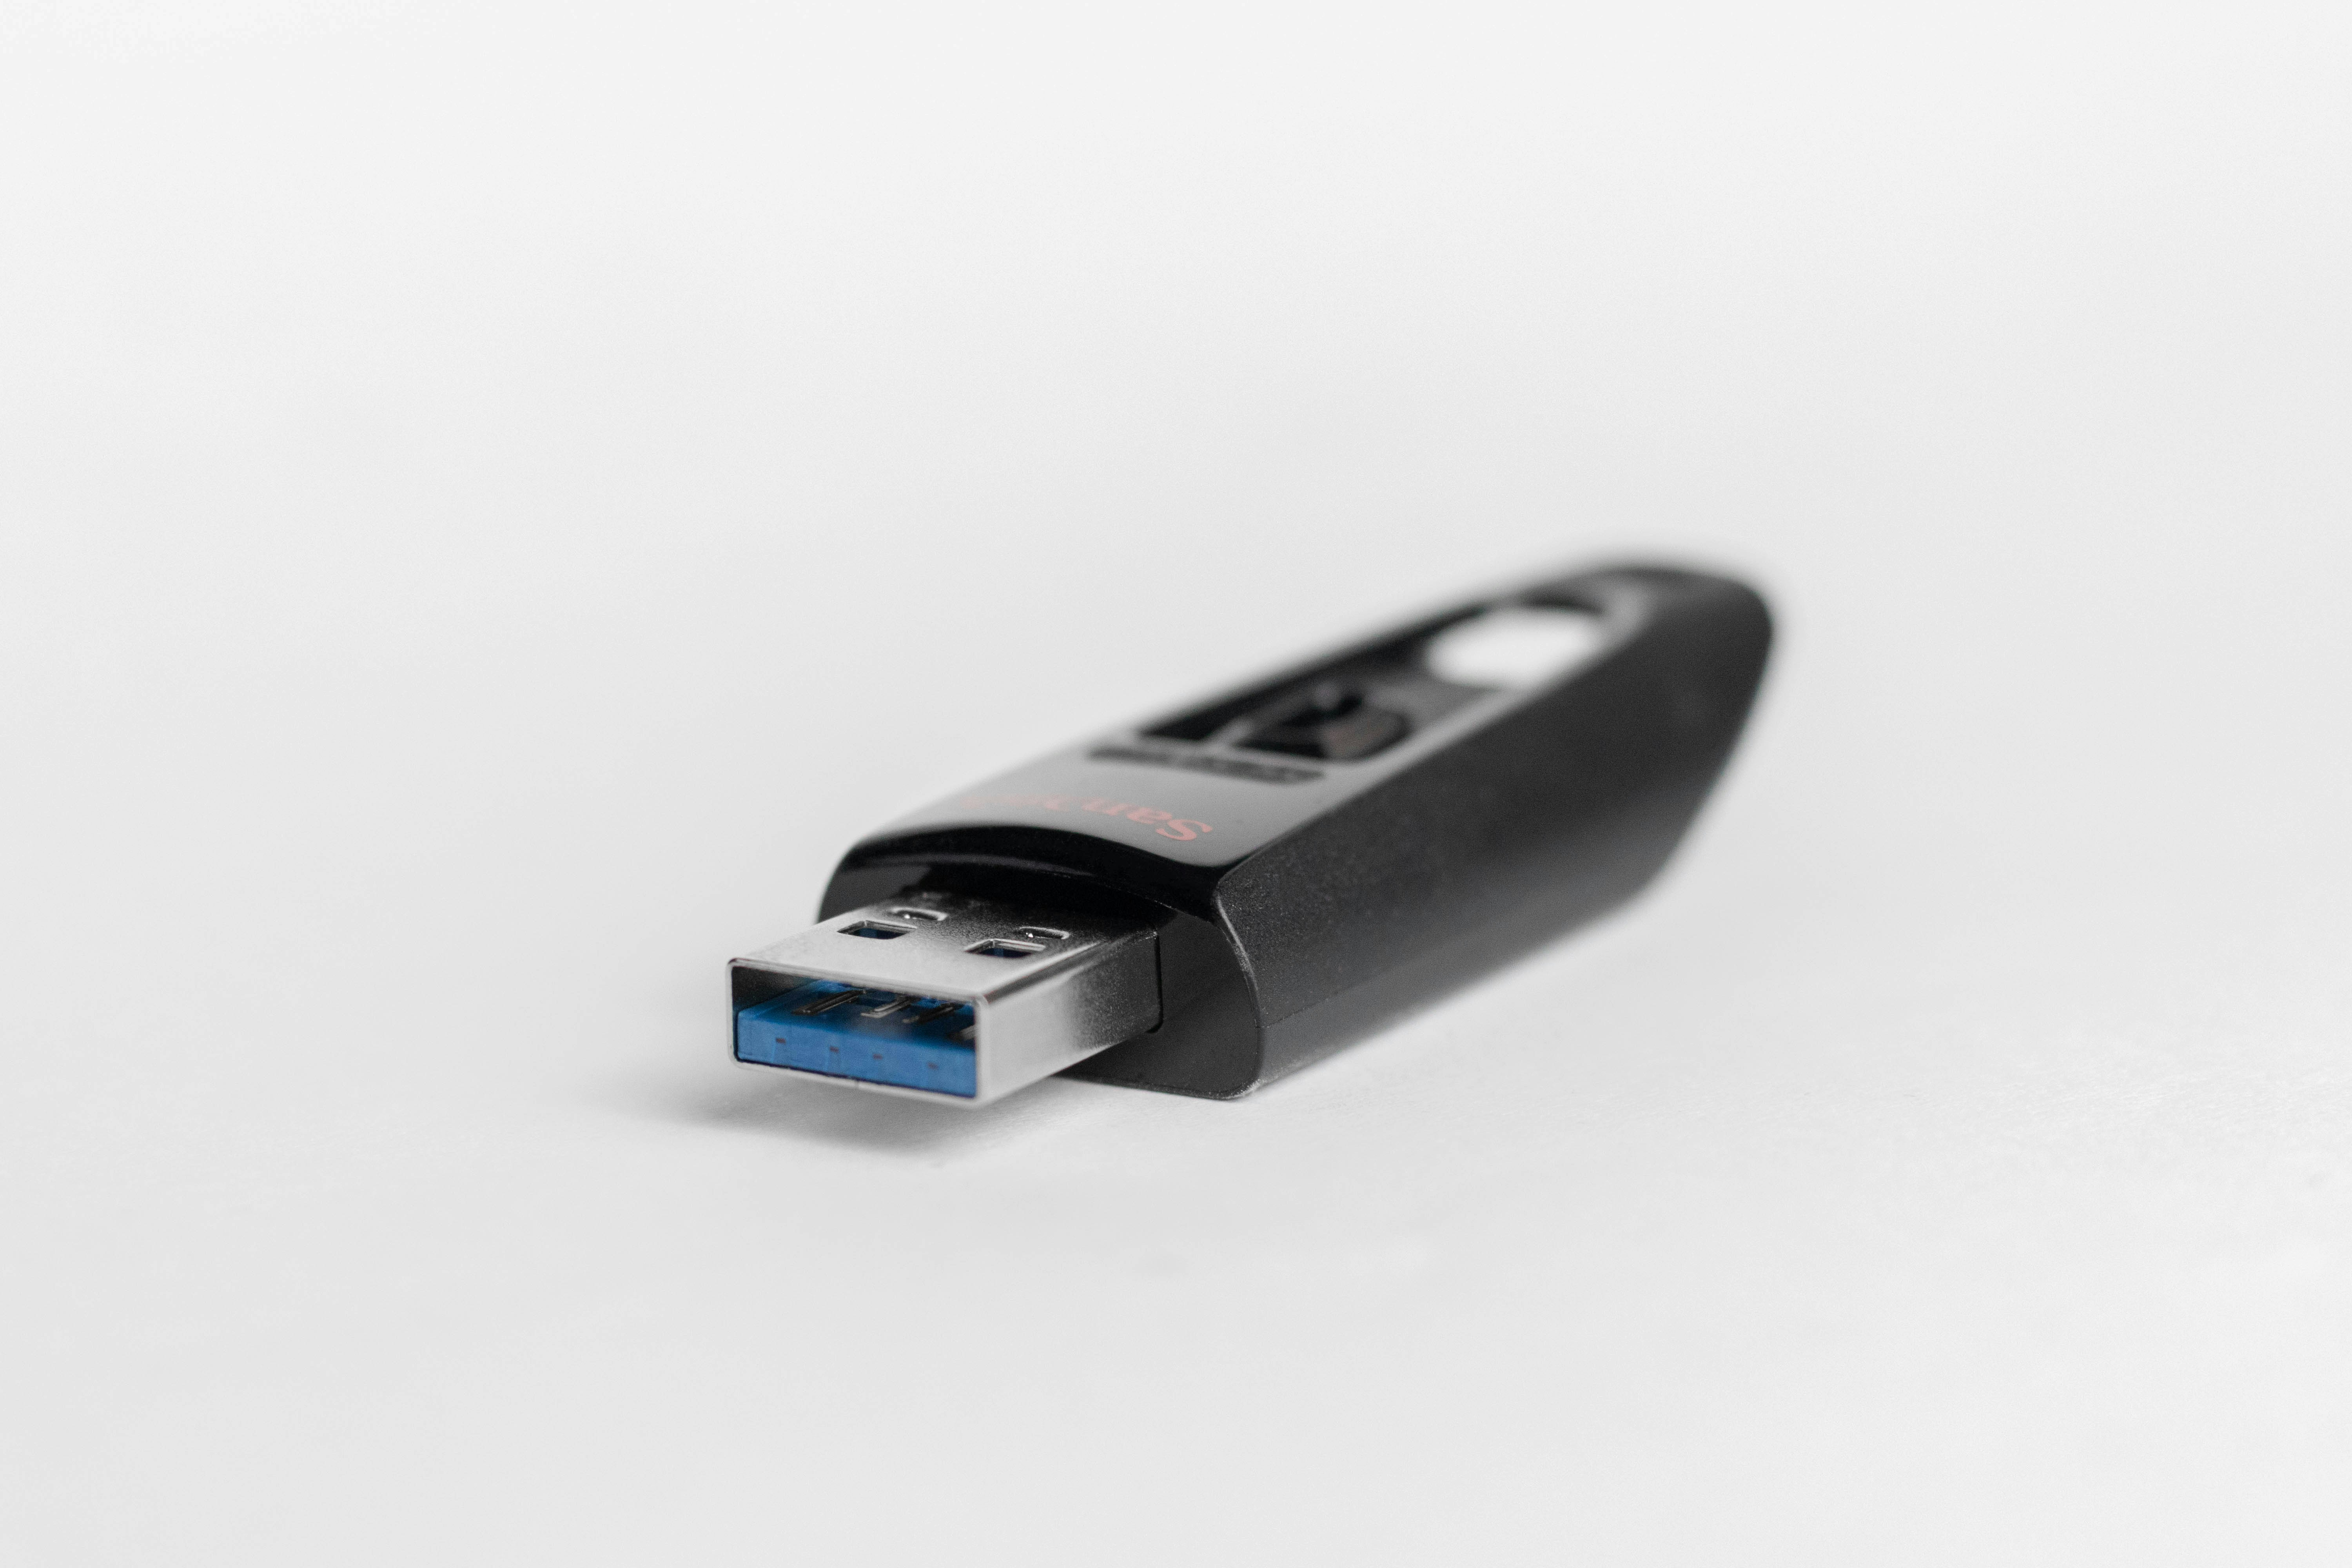
\includegraphics[width=\linewidth]{Im/thumb_drive.jpg}
				\onslide<3>
\includegraphics[width=\linewidth]{Im/discord.png}
				\onslide<4>
\includegraphics[width=\linewidth]{Im/cumulus.jpg}
			\end{overprint}
		\end{column}
	\end{columns}
\end{frame}

% add on the previous slide a small note telling that not all methods are equal
\begin{frame}[fragile]{donné et partage de fichiers}
	\begin{itemize}
		\item photo de l'écran
		\item une clé USB
		\item fichier sur discord
		\item Cloud (google drive, dropbox, \dots)
	\end{itemize}
	% add a note that not all methods are equal
	\begin{alertblock}{Attention}
		Toutes les méthodes ne se valent pas !
	\end{alertblock}
\end{frame}

\begin{frame}[fragile]{donné et partage de fichiers}
	%create a comand for the red ding{55} and green checkmark
	\resizebox{\linewidth}{!}{
		\begin{tabular}{|l|c|c|c|c|c|c|}
			\hline
			\textbf{Méthode} & \textbf{Historique} & \textbf{Sauvegarde} & \textbf{Collaboration} & \textbf{Travail en parallèle} & \textbf{Commentaires} & \textbf{Automatisation} \\ \hline
			\hline
			\textbf{Prendre une photo} & \redx & \redx & \redx & \redx & \redx & \redx \\ \hline
			\textbf{Clé USB} & \redx & \greenv & \redx & \redx & \redx & \redx \\ \hline
			\textbf{Serveur Discord} & \redx & \greenv & \greenv & \redx & \redx & \redx \\ \hline

			\textbf{Cloud} & \greenv & \greenv & \greenv & \redx & \greenv & \redx \\ \hline
		\end{tabular}
	}
\end{frame}

% now we will show the advantages and disadvantages of each of the methods using tables each line will be a method and the columns will a thing to do and the cell will be a cross or a checkmark
\begin{frame}[fragile]{donné et partage de fichiers}
	%create a comand for the red ding{55} and green checkmark
	\resizebox{\linewidth}{!}{
		\begin{tabular}{|l|c|c|c|c|c|c|}
			\hline
			\textbf{Méthode} & \textbf{Historique} & \textbf{Sauvegarde} & \textbf{Collaboration} & \textbf{Travail en parallèle} & \textbf{Commentaires} & \textbf{Automatisation} \\ \hline
			\hline
			\textbf{Prendre une photo} & \redx & \redx & \redx & \redx & \redx & \redx \\ \hline
			\textbf{Clé USB} & \redx & \greenv & \redx & \redx & \redx & \redx \\ \hline
			\textbf{Serveur Discord} & \redx & \greenv & \greenv & \redx & \redx & \redx \\ \hline
			\textbf{Cloud} & \greenv & \greenv & \greenv & \redx & \greenv & \redx \\ \hline
			\textbf{Git (VCS)} & \greenv & \greenv & \greenv & \greenv & \greenv & \greenv \\ \hline
		\end{tabular}
	}
\end{frame}
		
\begin{frame}[fragile]{Introduction à Git}
	\begin{itemize}
		\item Comment ça marche ?
		\item Quels sont les avantages ?
		\item Comment l'installer ?
		\item Comment l'utiliser ?
		\item Exercices pratiques
	\end{itemize}
\end{frame}


\begin{frame}[fragile]{Comment ça marche ?}{test}
	
	Git est un système de contrôle de version (VCS) distribué, un VCS est une base de données qui utilise un système de fichiers pour enregistrer les modifications apportées à un ensemble de fichiers utilisent la théorie des graphes... BREF !
\end{frame}

\begin{frame}[fragile]{Comment ça marche ?}
	comme xkcd le dit si bien...
	%add the xkcd comic about git on the entire slide
	\begin{center}
		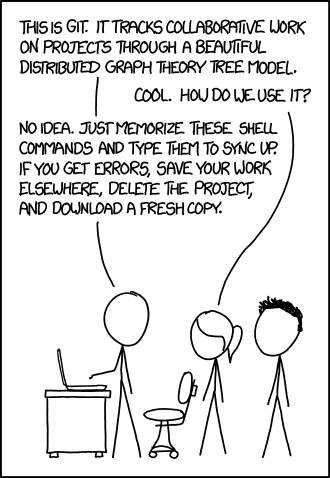
\includegraphics[width=0.4\linewidth]{Im/git_xkcd.png}
	\end{center}
\end{frame}

\begin{frame}[fragile]{Comment ça marche ?}
	\framesubtitle{Comment ça marche ?}
	
	%spongebob meme about magic 
	git est magic!
	\begin{center}
		
\includegraphics[width=0.4\linewidth]{Im/its-a-kind-of-magic.jpg}
	\end{center}

	il peut faire tout ce que vous voulez, mais il faut savoir comment lui demander

\end{frame}

\begin{frame}{Quels sont les avantages ?}
	% \begin{column}{0.5\linewidth}
		en quoi git est-il mieux que les autres méthodes ?
		% \begin{column}{0.5\linewidth}
			\begin{itemize}
				\item <1-> Historique des modifications
				\item <2-> Sauvegarde
				\item <3-> Commentaires
				\item <4-> Automatisation
			\end{itemize}
		% \end{column}
		% \begin{column}{0.5\linewidth}	
			% \begin{overprint}
			% 	% on the first slide we will show the 2 screenshots of the code and the code modification and onder a 3rd image with the change in the code
			% 	\onslide<1>{
			% 		\begin{subcaptiongroup}
			% 			\begin{subfigure}{0.3\linewidth}
			% 				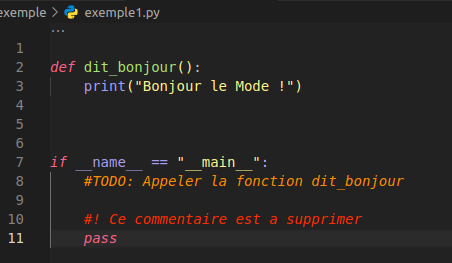
\includegraphics[width=\linewidth]{Im/exemple/pre_modif.png}
			% 				\caption{Code original}
			% 			\end{subfigure}
			% 			\begin{subfigure}{0.3\linewidth}
			% 				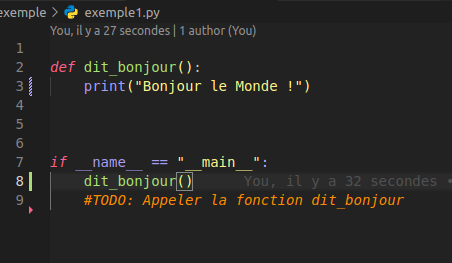
\includegraphics[width=\linewidth]{Im/exemple/post_modif.png}
			% 				\caption{Différence}
			% 			\end{subfigure}
			% 			\begin{subfigure}{0.3\linewidth}
			% 				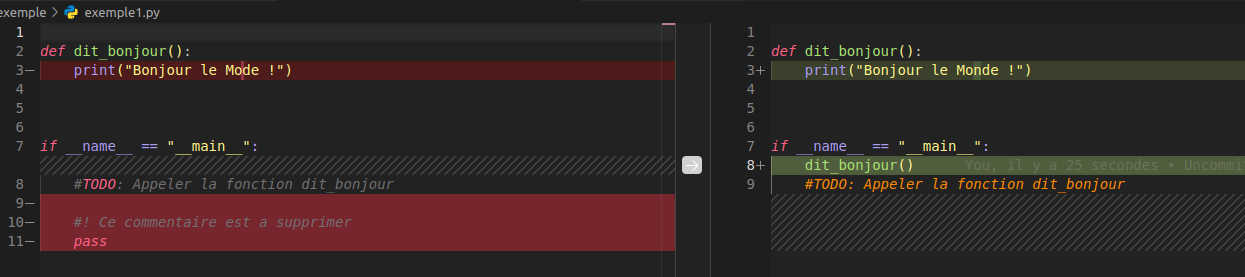
\includegraphics[width=\linewidth]{Im/exemple/modif_visualisation.png}
			% 				\caption{Code modifié}
			% 			\end{subfigure}
			% 		\end{subcaptiongroup}
			% 		}
			% \end{overprint}
		% \end{column}
	% \end{column}
\end{frame}
	
	


\begin{frame}[fragile]{Comment utilser ?}
	les commandes de base:
	\begin{itemize}
		\item git init
		\item git add
		\item git commit
	\end{itemize}

	les commandes un peu plus avancées (surtout utile en collaboration)
	\begin{itemize}
		\item git branch
		\item git checkout et git switch
		\item git merge
	\end{itemize}

	% bloc pour dire que on ne va que voir les commande sur la ligne de commande
	\begin{alertblock}{Note}
		Nous ne verrons que les commandes en ligne de commande, mais il existe des interfaces graphiques pour git (voir \ref{sec:aller-plus-loin})
	\end{alertblock}
\end{frame}


\begin{frame}[fragile]{les commandes de base}
	\begin{itemize}
		\item<1-3> git init
		\item <2-3> git add
		\item <3-3> git commit
	\end{itemize}

	\begin{onlyenv}<1>
		\begin{block}{git init}
			\texttt{git init} permet de créer un nouveau dépôt git dans le répertoire courant sous la forme d'un dossier caché \texttt{.git}
		\end{block}

		\begin{block}{note}
			\texttt{.git} n'as pas besoin d'être modifié directement, il est géré par git lui-même. mais si vous voulez automatiser des tâches, vous pouvez ajouter des scripts dans le dossier \texttt{.git/hooks}
		\end{block}

		commande à taper: \lstinline|git init|
	\end{onlyenv}

	\begin{onlyenv}<2>
		\begin{block}{git add}
			\texttt{git add} permet d'ajouter des fichiers à l'index de git, c'est-à-dire de dire à git que vous voulez suivre les modifications de ce fichier et % add color to the text
			quand vous ferez un commit, 
			\color{red}
			Uniquement
			\color{black}
			les modifications de ces fichiers seront prises en compte.
		\end{block}

		commande à taper: \lstinline|git add <fichier>| \\
		
		\texttt{<fichier>}: peut être un fichier ou un dossier
	\end{onlyenv}

	\begin{onlyenv}<3>
		\begin{block}{git commit}
			\texttt{git commit} permet de sauvegarder les modifications de vos fichiers dans le dépôt git. il est important de mettre un message clair et concis pour expliquer les modifications apportées.
		\end{block}

		commande à taper: \lstinline|git commit -m "message"| \\
		le -m est obligatoire et le message doit être entre guillemets
	\end{onlyenv}
\end{frame}
\begin{frame}
	Bravo vous avez fait votre premier commit !
	\pause
	\begin{center}
		
\includegraphics[width=0.5\linewidth]{Im/question-mark.png}
	\end{center}
\end{frame}


	% \begin{frame}[fragile]{Rust n'est pas \texttt{null}}
	% 	La \texttt{NullPointerException} est probablement l'exception la plus connue en Java.
	
	% 	\begin{lstlisting}[language=java]
	% User user = null;  // Valid Java
% user.greet();      // NullPointerException
% 	\end{lstlisting}
	
% 	En Rust, on utilise le type générique \texttt{Option<T>} pour représenter un type qui peut être \texttt{null}.
	
% 	\begin{lstlisting}
% let user1 = None;
% user1.greet(); // Ne compile pas
% let user2 = Some(User{name:"Yannick"});
% if let Some(u) = user2 {
%   u.greet();
% }
% \end{lstlisting}
% \end{frame}

% \begin{frame}[fragile]{Conséquences dans d'autres langages}
% 	Certains langages utilisent une syntaxe similaire à Rust. Java a introduit le type \texttt{Optional<T>} qui nécessite aussi d'être vérifié.
	
% 	Exemple en Python et utilité du type hinting.
% \end{frame}

% \begin{frame}[fragile]{Des objets complets}
% 	\begin{lstlisting}
% class User:
% 	age: int
% 	name: str
	
% 	def __init__(self, name):
% 		self.name = name

% u = User("Yannick")
% print(u.age)
% 	\end{lstlisting}
% 	\only{
% 		\begin{blueblock}{Est-ce possible en Rust ?}\end{blueblock}
% 	}<2>
% 	\only{\begin{blueblock}{Est-ce possible en Rust ?}
% 			Non, grace à son typage fort, Rust garantit que chaque attribut d'une structure correspond bel et bien au type indiqué.
% 		\end{blueblock}}<3>			
	
% \end{frame}



% \begin{frame}[fragile]{Ownership et mutabilité (1)}
% 	En regardant ce code Java, que peut-on dire de la variable \texttt{address} donnée en paramètre ?
% \begin{lstlisting}[language=Java]
% void setAddress(Address address) {
%   this.address = address;
% }	
% \end{lstlisting}
% 	\only{
% 	\begin{itemize}
% 		\item La méthode ne précise pas si la variable \texttt{address} est exclusivement utilisée par \texttt{this} ou si d'autres objets y ont accès.
% 		\item Si d'autres objets y ont accès, a-t-on le droit de modifier cette variable ?
% 	\end{itemize}}<2>
% \end{frame}

% \begin{frame}[fragile]{Valeur ou référence ?}
% 	En Python, Java ou JavaScript, (presque) tout se passe par référence.
	
% 	\begin{lstlisting}[language=Python]
% # Python
% def change_name(name: str):
%   self.name = name
% 	\end{lstlisting}
% 	\begin{lstlisting}[language=Java]
% // Java
% void setAddress(Address addr) {
%   this.address = addr;
% }	
% \end{lstlisting}
% 	Et rien ne montre de l'extérieur que ces fonctions modifient le contenu de l'utilisateur.	
% \end{frame}


% \begin{frame}[fragile]{Ownership et mutabilité (2)}
% 	En Rust, c'est explicite et vérifié à la compilation.
	
% 	\begin{lstlisting}
% change_address1(&mut self, address: &Address) {
%   self.address = address.clone();
% }

% change_address2(&mut self, address: Address) {
%   self.address = address;
% }

% change_address3(&mut self, address: &mut Address) {
%   address.postcode = 1050;
%   self.address = address.clone();
% }
% 	\end{lstlisting}
% \end{frame}

% \begin{frame}{Parallélisme}
% 	La modification concurrente d'une variable partagée est un problème récurrent dans le cadre du multi-threading (et du parallélisme plus généralement) ?
	
% 	\only{\begin{blueblock}{En quoi ce problème est-il lié à l'ownership ?}		
% 	\end{blueblock}}<2>
% 	\only{\begin{blueblock}{En quoi ce problème est-il lié à l'ownership ?}
% 		Si on donne l'ownership de plusieurs variables à plusieurs threads, alors chacun sait que lui seul possède la variable, et il ne peut pas y avoir de \textit{race condition}.
% 	\end{blueblock}}<3>
% \end{frame}

% \begin{frame}{Parallélisme (2)}
% 	Et si on veut quand-même modifier une variable partagée ?
	
% 	Alors on utilise le pattern d'\textit{interior mutability} avec une \texttt{Mutex<T>}.
	
% 	\begin{blueblock}{\textit{Interior mutability}}
% 		C'est un principe qui va permettre de modifier une variable interne sans montrer au compilateur qu'une modification a lieu. \texttt{Mutex<T>} utilise ce pattern.
% 	\end{blueblock}
% \end{frame}

% \begin{frame}[fragile]{Itérateurs parallèles}
% 	Rust propose beaucoup de fonctions sur les itérateurs.
	
% 	\begin{blueblock}{Itérateurs parallèles}
% 		Comme on sait ce qui appartient à qui, on sait aussi ce qu'on peut paralléliser !	
% 	\end{blueblock}
	
% 	\only{\begin{center}
% 			\includegraphics[width=\linewidth]{}
% 	\end{center}}<2>
% \end{frame}


% \begin{frame}{Ce dont on n'a pas encore parlé...}
% 	\begin{itemize}
% 		\item La puissance des \texttt{enum} et le pattern matching
% 		\item L'absence d'héritage
% 		\item La gestion des erreurs
% 		\item interopérabilité avec d'autres langages
% 		\item \texttt{cargo}
% 		\item Les autres projets (deno2, ruff, uv, \dots) qui exploitent les capacités de Rust
% 		\item La courbe d'apprentissage (oups !)
% 	\end{itemize}
% \end{frame}

% \begin{frame}{Conclusions}
% 	Rust vous contraint à respecter de nombreuses règles qui sont condiérées comme des \textit{bonnes pratiques} ou des \textit{edge cases} dans d'autres langages
% 	\begin{itemize}
% 		\item typage en Python
% 		\item clone ou pas clone ?
% 		\item muable ou immuable ?
% 		\item \texttt{free} ou pas \texttt{free} ? 
% 	\end{itemize}
% \end{frame}

\end{document}
